\documentclass[11pt,a4paper]{article}
\usepackage{tikz}
	
\title{\huge \bold {FufGUx} (Building CPU on breadboards \textit{only} using logic gates)}
\author{coding, lothar}

\begin{document}
	
	\begin{titlepage}
		
		\clearpage
		\maketitle
		\thispagestyle{empty}
		
	\end{titlepage}

	\section{Modus operandi}
	
	
	We basically just make CPU n shit and we don't care bout copyright n shit because it not really relevant here. We just steal, we just salvage, we don't give a shit.
	
	\vspace{1cm}
	
	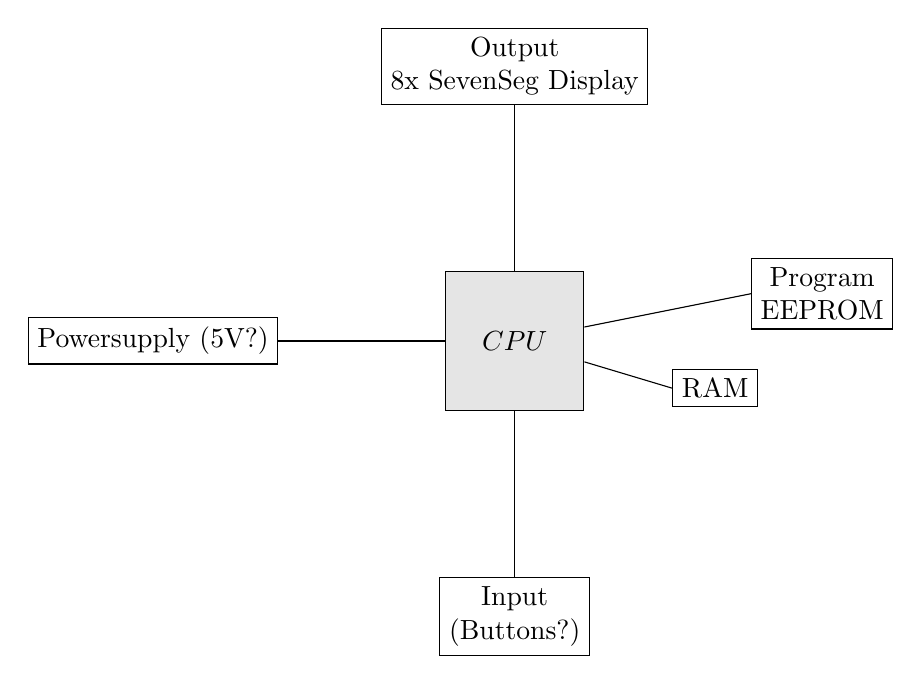
\begin{tikzpicture}
		
		\node [draw, fill=black!10, minimum size=50] (c) {$CPU$};
		
		\draw (c)--(-3,0) node[draw, align=center, left]{Powersupply (5V?)};		
		
		\draw (c)--(0,3) node[draw, align=center, above]{Output\\8x SevenSeg Display};		
		
		\draw (c)--(3,0.6) node[draw, align=center, right]{Program\\EEPROM};
		\draw (c)--(2,-0.6) node[draw, align=center, right]{RAM};	
		
		\draw (c)--(0,-3) node[draw, align=center, below]{Input\\(Buttons?)};
		
	\end{tikzpicture}

	\vspace{1cm}

	so uhm jeh dis is basikly the basic stuff we wanna make so yes...

\end{document}